\documentclass{article}
\usepackage[letterpaper, margin=1.25in, left=1.25in]{geometry}
\usepackage{datetime}
\usepackage{tocloft}
\usepackage{fancyhdr}
\usepackage{nomencl}

% Table:
\usepackage{float}
\usepackage[table,xcdraw]{xcolor}
\usepackage{tabularx}
\newcolumntype{Y}{>{\centering\arraybackslash}X}
\usepackage[singlelinecheck=false]{caption}

% Figures:
\usepackage{graphicx}
\usepackage[export]{adjustbox}

%%%%%%%%%%%%%%%%%%%%%%%%%%%%%%%%%%%%%%%%%%%%%%%%%%%%%%%%%%%%%%%%%%%%%%%%%%%%%%%%
% Customizations
% --------------
\makeatletter
% Quoting
\newcommand{\quotes}[1]{``#1"}

% Add dots to table of contents
\renewcommand{\cftsecleader}{\cftdotfill{\cftdotsep}}

% Remove self reference/title
\let\@cftmaketoctitle\relax
\let\@cftmakelottitle\relax
\let\@cftmakeloftitle\relax
\makeatother

% position page number to bottom right
\fancyhf{}
\renewcommand{\headrulewidth}{0pt}
\rfoot{\thepage}
\pagestyle{fancy}

% Make List of Abbrev into section
\renewcommand{\nomname}{List of Abbreviations}
\patchcmd{\thenomenclature}{\section*}{\section}{}{}

%%%%%%%%%%%%%%%%%%%%%%%%%%%%%%%%%%%%%%%%%%%%%%%%%%%%%%%%%%%%%%%%%%%%%%%%%%%%%%%%
% Title Page
% ----------
\makeatletter
\newcommand{\thesistitle}{Characterization of the human thyroid epigenome}
\newcommand{\studentname}{Celia Siu}
\newcommand{\previousdegree}{B.Sc., The University of British Columbia, 2013}
\newcommand{\degreename}{Master of Science}
\newcommand{\program}{Bioinformatics}
\newcommand{\campus}{Vancouver}
\newcommand{\gradmonth}{\monthname}  % Prints current month
\newcommand{\gradyear}{\the\year}    % Prints current year

\renewcommand{\maketitle}{
	\begin{titlepage}
	\null\vfil\par
	\begin{center}\setlength{\baselineskip}{20pt}
		{\Large \textbf{\thesistitle}}\\[1em]

		{\Large by}\\[1em]
		{\Large \studentname}\\[1em]
		{\Large \previousdegree}\\[1em]

		{\Large \textsc{A thesis submitted in partial fulfillment of}}\\
		{\Large \textsc{the requirements for the degree of}}\\[1em]

		{\Large \textbf{\degreename}}\\[1em]
		{\Large in}\\[1em]
		{\Large \textsc{The Faculty of Graduate and Postdoctoral Studies}}\\[1em]
		{\Large (\program)}\\[1em]

		{\Large The University of British Columbia}\\
		{\Large (\campus)}\\[1em]
		{\Large \gradmonth\ \gradyear}\\[1em]
		{\Large \textcopyright\ \studentname, \gradyear}
	\end{center}
	\vfill\null
	\end{titlepage}
}
\makeatother

%%%%%%%%%%%%%%%%%%%%%%%%%%%%%%%%%%%%%%%%%%%%%%%%%%%%%%%%%%%%%%%%%%%%%%
% Order of components
% -------------------
\begin{document}

% 1. TITLE PAGE (required)
\maketitle

% 2. ABSTRACT (required - max 350 words)
\pagenumbering{roman}
\setcounter{page}{2}
\section{Abstract}
The abstract is a concise and accurate summary of the scholarly work described in the document. It states the problem, the methods of investigation, and the general conclusions, and should not contain tables, graphs, complex equations, or illustrations. There is a single scholarly abstract for the entire work, and it must not exceed 350 words in length.

%%%%%%%%%%%%%%%%%%%%%%%%%%%%%%%%%%%%%%%%%%%%%%%%%%%%%%%%%%%%%%%%%%%%%%%%%%%%%%%%
\pagebreak
\section{Lay summary}
{\it Effective May 2017, all theses and dissertations must include a lay summary.}

The lay or public summary explains the key goals and contributions of the research/scholarly work in terms that can be understood by the general public. it does not use technical terms and discipline-specific language. It must not exceed 150 words in length.


% % 3. PREFACE (required)
\section{Preface}
The Preface must include a statement indicating the student's contribution to the following:
\begin{itemize}
  \item Identification and design of the research program,
  \item Performance of the various parts of the research, and
  \item Analysis of the research data.
\end{itemize}

\begin{flushleft}Certain additional elements may also be required, as specified below.\end{flushleft}
\begin{itemize}
  \item If any of the work presented in the thesis has led to any publications or submissions, all of these must be listed in the Preface. Bibliographic details should include the title of the article and the name of the publisher (if the article has been accepted or published), and the chapter(s) of the thesis in which the associated work is located.
  \item If the work includes publications or material submitted for publication, the statement described above must detail the relative contributions of all collaborators and co-authors (including supervisors and members of the supervisory committee) and state the proportion of research and writing conducted by the student. For further details, see “Including Published Material in a Thesis or Dissertation”.
  \item If the work includes other scholarly artifacts (such as film and other audio, visual, and graphic representations, and application-oriented documents such as policy briefs, curricula, business plans, computer and web tools, pages, and applications, etc.), all of these must be listed in the Preface (with bibliographical information, if applicable).
\end{itemize}

If ethics approval was required for the research, the Preface must name the responsible UBC Research Ethics Board, and report the project title(s) and the Certificate Number(s) of the Ethics Certificate(s) applicable to the project.

In a thesis where the research was not subject to ethics review, produced no publications, and was designed, carried out, and analyzed by the student alone, the text of the Preface may be very brief. Samples are available on this website and in the University Library's online repository of accepted theses.

The content of the Preface must be verified by the student's supervisor, whose endorsement must appear on the final Thesis/Dissertation Approval form.

Acknowledgements, introductory material, and a list of publications do not belong in the Preface. Please put them respectively in the Acknowledgements section, the first section of the thesis, and the appendices.


% 4. TABLE OF CONTENTS (required - will be generated for you)
\pagebreak
\section{Table of Contents}
\tableofcontents

% 5. LIST OF TABLES (required - will be generated for you)
\pagebreak
\section{List of Tables}
\listoftables

% 6. LIST OF FIGURES (required - will be generated for you)
\pagebreak
\section{List of Figures}
\listoffigures

% 7. LIST OF ILLUSTRATIONS (required if document has illustrations)
% As I did not have illustrations in my thesis,
% you will need to set this up if you do.

% 8. LISTS OF SYMBOLS, ABBREVIATIONS OR OTHER (advisable)
% We use the "nomencl" package to create the list of abbreviations
% The section header is already produced by this package,
% so we do not declare it again

\makenomenclature % to produce *.nlo file

% You will need to add entries e.g.
\nomenclature{UBC}{University of British Columbia}

% and compile:
%   makeindex $*.nlo -s nomencl.ist -o $*.nls

\printnomenclature[1in]


% 9. GLOSSARY (optional)

% 10. ACKNOWLEDGEMENTS (optional)
\section{Acknowledgements}

Students may include a brief statement acknowledging the contribution to their research and studies from various sources, including (but not limited  to)
\begin{itemize}
  \item Their research supervisor and committee,
  \item Funding agencies,
  \item Professional or community collaborators,
  \item Fellow students, and
  \item Family and friends.
\end{itemize}


% 11. DEDICATION (optional)

% 12. INTRODUCTION
% 13. RESEARCH CHAPTERS
% 14. CONCLUSION
\pagebreak
\pagenumbering{arabic}
% Body of Thesis

%%%%%%%%%%%%%%%%%%%%%%%%%%%%%%%%%%%%%%%%%%%%%%%%%%%%%%%%%%%%%%%%%%%%%%%%%%%%%%%%
% A. Introduction
% ---------------
\section{Introduction}
The thesis must clearly state its theme, hypotheses and/or goals (sometimes called “the research question(s)”), and provide sufficient background information to enable a non-specialist scholar to understand them. It must contain a thorough review of relevant literature, perhaps in a separate chapter.


%%%%%%%%%%%%%%%%%%%%%%%%%%%%%%%%%%%%%%%%%%%%%%%%%%%%%%%%%%%%%%%%%%%%%%%%%%%%%%%%
% B. Research Chapters
% --------------------

% We can define variables and colors to be referenced later
\newcommand{\numberofsamples}{4}
\newcommand{\sampleA}{CEMT\_40}
\newcommand{\sampleB}{CEMT\_42}
\newcommand{\sampleC}{CEMT\_44}
\definecolor{tableheader}{HTML}{EFEFEF}
\definecolor{colorstate1}{RGB}{255,0,0}

\section{Research chapters}

The account of the scholarly work should be presented in a manner suitable for the field. It should be complete, systematic, and sufficiently detailed to enable a reader to understand how the data were gathered and analyzed, and how to apply similar methods in another study. Notation and formatting must be consistent throughout the thesis, including units of measure, abbreviations, and the numbering scheme for tables, figures, footnotes, and citations. One or more chapters may consist of material published (or submitted for publication) elsewhere, or other artifacts (e.g., film, application-oriented documents) placed in a scholarly context. See “Including Published Material in a Thesis or Dissertation” for additional details.

\subsection{Data}
\subsection{Methods}
\subsubsection{Method 1}
\subsubsection{Method 2}
\subsubsection{Method 3}
\subsection{Results}
\subsubsection{Result 1}

In Figure~\ref{fig:fig1}, we show a spectrum.

\begin{figure}[H]
  \centering
  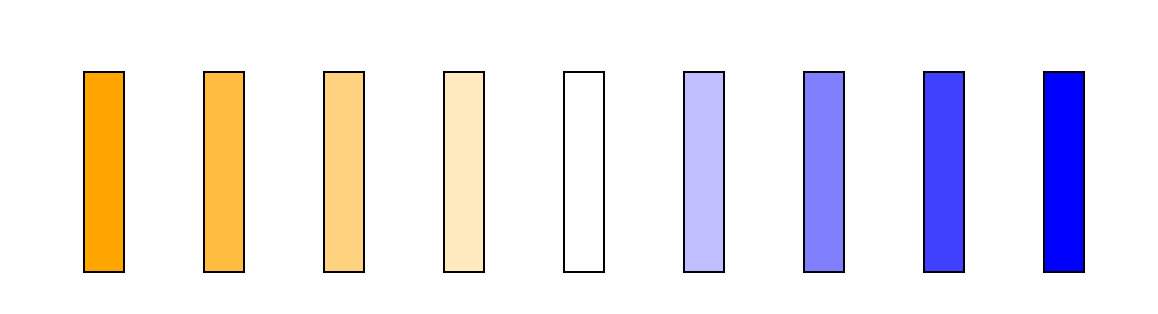
\includegraphics[width=0.75\textwidth]{figures/fig1.png}
  \vspace{-.5em}
  \caption{\nbars~bars}
  \label{fig:fig1}
\end{figure}

\subsubsection{Result 2}
\subsubsection{Result 3}


%%%%%%%%%%%%%%%%%%%%%%%%%%%%%%%%%%%%%%%%%%%%%%%%%%%%%%%%%%%%%%%%%%%%%%%%%%%%%%%%
% C. Conclusion
% -------------
\section{Conclusion}
In this section the student must demonstrate his/her mastery of the field and describe the work's overall contribution to the broader discipline in context. A strong conclusion includes the following:

\begin{itemize}
  \item Conclusions regarding the goals or hypotheses presented in the Introduction,
  \item Reflective analysis of the scholarly work and its conclusions in light of current knowledge in the field,
  \item Comments on the significance and contribution of the scholarship reported,
  \item Comments on strengths and limitations of the research/scholarship,
  \item Discussion of any potential applications of the findings, and
  \item A description of possible future research directions, drawing on the work reported.
\end{itemize}



% 15. BIBLIOGRAPHY (required)
% Note: you need to \cite{...} before this section gets generated
% Examples are added in acknowledgements.tex
\pagebreak
\section{References}
\renewcommand{\section}[2]{}
\bibliographystyle{plain}
\bibliography{references/biblio}

% 16. APPENDICES

\end{document}
